\chapter{Qualitätsmanagement}
	\begin{figure}[H]
		\centering
		{\tiny
			\csvautotabular{../qualityManagement/timelog.csv}
		}
		\caption{Die Aktivität ``Qualitätsmanagement"' fasst Testing und Reviewing
		zusammen.}
	\end{figure}


	\section{Unittests}		
		\begin{figure}[H]
			\centering
			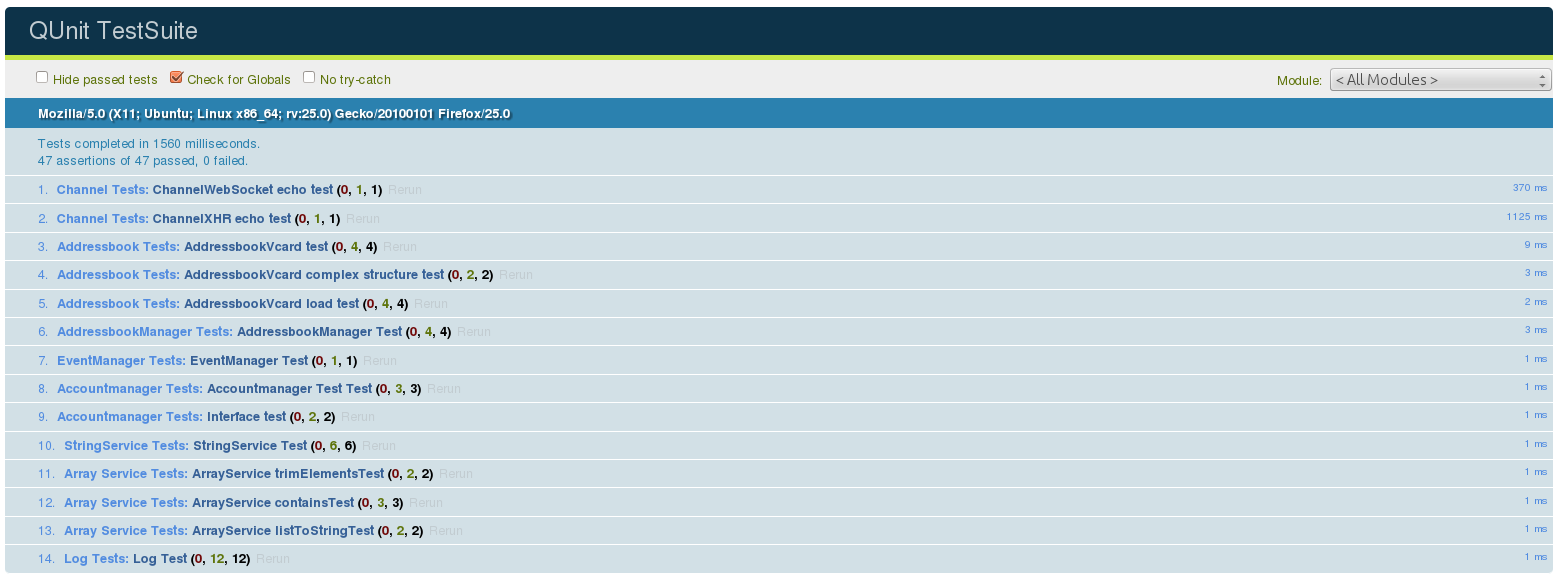
\includegraphics[width=1\textwidth]{../qualityManagement/unittesting.png}
			\label{unittests}
		\end{figure}
		Die Applikationsdomain wird mit Unittests getestet und die fortbleibende
		Funktion bei Änderungen damit nachgewiesen.
		
	\section{Performancetests}
		Die Performance wird durch eine umfangreiche Performanceanalyse untersucht und dokumentiert.
		
		Siehe Anhang \ref{performanceanalyse}
		
	\section{Funktionstests}
		Die Funktion der Applikation als Gesamtes wird durch regelmässige, auch
		Browser- und Betriebssystem-übergreifende, manuelle Tests gewährleistet.
		
	\section{Reviews}
		Regelmässige Reviews stellen die Qualität von Dokumentation und Code sicher. Für die Reviews wird die Commit-Kommentarfunktion von GitHub genutzt.
